\documentclass[12pt,a4paper]{article}
\usepackage[utf8]{vietnam}
\usepackage{amsmath,amssymb,amsfonts,mathrsfs}
\usepackage[left=1.5cm,right=1.5cm,top=2cm,bottom=2cm,headheight=17pt]{geometry}
\usepackage{enumitem}
\usepackage{array}
\usepackage{graphicx}
\usepackage{fancyhdr}

\pagestyle{fancy}
\fancyhf{}
\lhead{\small\textbf{HƯỚNG TỚI THPTQG 2027}}
\rhead{\small\textit{Người biên soạn: Dương Gia Bảo}}
\rfoot{\small Trang \thepage}
\renewcommand{\headrulewidth}{0.4pt}

\begin{document}

\noindent
\begin{minipage}[t]{0.40\textwidth}
    \centering
    \textbf{HƯỚNG TỚI THPTQG 2027}\\[-2pt]
    \rule{3.2cm}{0.6pt}\\[4pt]
    \textbf{ĐỀ CHÍNH THỨC}
\end{minipage}\hfill
\begin{minipage}[t]{0.58\textwidth}
    \centering
    \textbf{ĐỀ THI KHẢO SÁT CHẤT LƯỢNG}\\
    \textbf{ĐỀ SỐ 5}\\
    \textbf{Môn thi: TOÁN}\\
    \textit{\small Thời gian làm bài: 90 phút, không kể thời gian phát đề}
\end{minipage}

\vspace{0.2cm}
\noindent
\begin{minipage}[b]{0.78\textwidth}
    \textbf{Họ và tên:}\dotfill\textbf{SBD:}\makebox[3.5cm]{\dotfill}
\end{minipage}\hfill
\begin{minipage}[b]{0.20\textwidth}
    \hfill
    \setlength{\fboxrule}{0.8pt}%
    \fbox{\begin{minipage}{2.3cm}
        \centering
        \textbf{\small Mã đề thi}\\
        \textbf{0005}
    \end{minipage}}
\end{minipage}
\vspace{0.2cm}

% ==========================================
% PHẦN I
% ==========================================
\section*{\large PHẦN I. CÂU TRẮC NGHIỆM NHIỀU PHƯƠNG ÁN LỰA CHỌN}
\textit{Thí sinh trả lời từ câu 1 đến câu 12. Mỗi câu hỏi thí sinh chỉ chọn một phương án. Mỗi câu trả lời đúng được 0,25 điểm.}

\begin{enumerate}[label=\textbf{Câu \arabic*:}, leftmargin=*]

\item Cho hàm số $y = \dfrac{x^2 - x + 1}{x - 1}$ có đồ thị là $(C)$. Độ dài đoạn thẳng nối hai điểm cực trị của đồ thị hàm số $(C)$ bằng
\begin{enumerate}[label=\Alph*.]
    \item $2\sqrt{5}$.
    \item $4\sqrt{2}$.
    \item $\sqrt{10}$.
    \item $2\sqrt{3}$.
\end{enumerate}

\item Cho hàm số bậc ba $y = \dfrac{1}{3}x^3 - mx^2 + (m^2 - 4)x + 3$ với $m$ là tham số thực. Có bao nhiêu giá trị nguyên của $m \in [-10; 10]$ để hàm số có hai điểm cực trị $x_1, x_2$ thỏa mãn điều kiện $x_1^2 + x_2^2 = 26$?
\begin{enumerate}[label=\Alph*.]
    \item $1$.
    \item $4$.
    \item $2$.
    \item $0$.
\end{enumerate}

\item Có bao nhiêu giá trị nguyên của tham số $m \in [-10; 10]$ để bất phương trình $\log_2(x^2 - 2x + m) \le 3$ nghiệm đúng với mọi số thực $x \in [0; 2]$?
\begin{enumerate}[label=\Alph*.]
    \item $6$.
    \item $7$.
    \item $8$.
    \item $5$.
\end{enumerate}

\item Một chất điểm chuyển động theo phương thẳng đứng với gia tốc phụ thuộc thời gian $a(t) = 12 - 3t\text{ (m/s}^2\text{)}$ ($t \ge 0$). Biết vận tốc ban đầu tại thời điểm $t = 0$ bằng $0\text{ m/s}$. Quãng đường chất điểm di chuyển từ thời điểm $t = 0$ đến khi vận tốc đạt giá trị lớn nhất bằng
\begin{enumerate}[label=\Alph*.]
    \item $48\text{ m}$.
    \item $72\text{ m}$.
    \item $56\text{ m}$.
    \item $64\text{ m}$.
\end{enumerate}

\item Trong không gian $Oxyz$, cho hai điểm $A(1; 2; -1)$ và $B(3; 0; 3)$. Điểm $C(0; 0; z_0)$ thuộc trục $Oz$ sao cho tam giác $ABC$ vuông tại $C$. Tổng các giá trị có thể có của $z_0$ bằng
\begin{enumerate}[label=\Alph*.]
    \item $2$.
    \item $-2$.
    \item $4$.
    \item $0$.
\end{enumerate}

\item Một thành phố có dân số hiện tại là $2$ triệu người. Tỉ lệ tăng dân số hàng năm được duy trì ổn định ở mức $1{,}5\%$/năm. Hỏi sau ít nhất bao nhiêu năm thì dân số thành phố sẽ vượt quá $2{,}5$ triệu người lần đầu tiên?
\begin{enumerate}[label=\Alph*.]
    \item $14\text{ năm}$.
    \item $16\text{ năm}$.
    \item $15\text{ năm}$.
    \item $17\text{ năm}$.
\end{enumerate}

\item Khảo sát thời gian hoàn thành một bài thực hành (phút) của 40 học sinh thu được bảng số liệu ghép nhóm sau:
\begin{center}
\begin{tabular}{|c|c|c|c|c|}
\hline
\textbf{Thời gian (phút)} & $[10; 14)$ & $[14; 18)$ & $[18; 22)$ & $[22; 26)$ \\ \hline
\textbf{Số học sinh} & $6$ & $14$ & $16$ & $4$ \\ \hline
\end{tabular}
\end{center}
Độ lệch chuẩn $s$ của mẫu số liệu ghép nhóm trên bằng bao nhiêu (làm tròn kết quả đến hai chữ số thập phân)?
\begin{enumerate}[label=\Alph*.]
    \item $3{,}15\text{ phút}$.
    \item $3{,}46\text{ phút}$.
    \item $3{,}82\text{ phút}$.
    \item $2{,}95\text{ phút}$.
\end{enumerate}

\item Cho hai biến cố $A$ và $B$ thỏa mãn $P(A) = 0{,}6$, $P(B) = 0{,}5$ và $P(A \cup B) = 0{,}8$. Xác suất có điều kiện $P(A|\overline{B})$ của biến cố $A$ khi biết biến cố $B$ không xảy ra bằng
\begin{enumerate}[label=\Alph*.]
    \item $0{,}4$.
    \item $0{,}5$.
    \item $0{,}3$.
    \item $0{,}6$.
\end{enumerate}

\item Cho hàm số $y = \dfrac{x - 1}{x^2 - 2mx + 4}$. Có bao nhiêu giá trị nguyên của tham số $m \in [-5; 5]$ để đồ thị hàm số có đúng $3$ đường tiệm cận?
\begin{enumerate}[label=\Alph*.]
    \item $8$.
    \item $7$.
    \item $6$.
    \item $9$.
\end{enumerate}

\item Tập nghiệm của bất phương trình mũ $3^{x^2 - 4x} < 27$ là khoảng $(a; b)$. Giá trị của $a + b$ bằng
\begin{enumerate}[label=\Alph*.]
    \item $3$.
    \item $4$.
    \item $-4$.
    \item $5$.
\end{enumerate}

\item Trong không gian $Oxyz$, phương trình mặt cầu $(S)$ có tâm $I(2; -1; 0)$ và đi qua điểm $A(1; 1; 2)$ là
\begin{enumerate}[label=\Alph*.]
    \item $(x - 2)^2 + (y + 1)^2 + z^2 = 9$.
    \item $(x + 2)^2 + (y - 1)^2 + z^2 = 9$.
    \item $(x - 2)^2 + (y + 1)^2 + z^2 = 3$.
    \item $(x - 1)^2 + (y - 1)^2 + (z - 2)^2 = 9$.
\end{enumerate}

\item Thể tích $V$ của khối tròn xoay thu được khi quay hình phẳng giới hạn bởi đồ thị hàm số $y = (x-1)e^x$, trục hoành và hai đường thẳng $x = 1, x = 2$ xung quanh trục $Ox$ bằng
\begin{enumerate}[label=\Alph*.]
    \item $\dfrac{\pi(e^4 + e^2)}{4}$.
    \item $\dfrac{\pi(e^4 - 2e^2)}{4}$.
    \item $\dfrac{\pi(e^4 + 1)}{4}$.
    \item $\dfrac{\pi(e^4 - e^2)}{4}$.
\end{enumerate}

\end{enumerate}

% ==========================================
% PHẦN II
% ==========================================
\section*{PHẦN II. CÂU TRẮC NGHIỆM ĐÚNG/SAI}
\textit{Thí sinh trả lời từ câu 1 đến câu 4. Trong mỗi ý a), b), c), d) ở mỗi câu, thí sinh chọn Đúng hoặc Sai.}

\begin{enumerate}[label=\textbf{Câu \arabic*:}, leftmargin=*]

\item Một doanh nghiệp sản xuất $x$ trăm thùng phuy hóa chất chuyên dụng mỗi tháng ($0 < x \le 20$). Chi phí sản xuất $x$ trăm thùng phuy là $C(x) = x^3 - 9x^2 + 60x + 40$ (triệu đồng). Giá bán mỗi trăm thùng phuy phụ thuộc vào lượng cung ứng theo hàm giá $p(x) = 111 - 3x$ (triệu đồng/trăm thùng phuy). Nhà nước đánh thuế môi trường $15$ triệu đồng trên mỗi trăm thùng phuy bán ra. Lợi nhuận ròng của doanh nghiệp là $L(x) = R(x) - C(x) - 15x$ (triệu đồng), trong đó $R(x) = x \cdot p(x)$ là tổng doanh thu.
\begin{enumerate}[label=\alph*)]
    \item Tổng doanh thu khi bán hết $x$ trăm thùng phuy hóa chất là $R(x) = 111x - 3x^2$ (triệu đồng).
    \item Hàm lợi nhuận ròng hàng tháng của doanh nghiệp được cho bởi $L(x) = -x^3 + 6x^2 + 36x - 40$ (triệu đồng).
    \item Khi doanh nghiệp sản xuất và tiêu thụ $4$ trăm thùng phuy mỗi tháng ($x = 4$), mức lợi nhuận ròng thu được bằng $150$ triệu đồng.
    \item Doanh nghiệp đạt lợi nhuận ròng lớn nhất khi sản xuất $6$ trăm thùng phuy mỗi tháng và mức lợi nhuận lớn nhất bằng $176$ triệu đồng.
\end{enumerate}

\item Một thiết bị bay nghiên cứu khí quyển được phóng thẳng đứng lên không trung từ mặt đất. Kể từ thời điểm phóng $t = 0$ (giây), động cơ đẩy gia tốc thiết bị với hàm gia tốc $a(t) = 18t - 6t^2\text{ (m/s}^2\text{)}$ cho đến khi ngắt động cơ tại thời điểm $t = 3$ giây. Sau $t = 3$ giây, thiết bị chuyển động chậm dần đều dưới tác dụng của trọng lực với gia tốc trọng trường $g = 10\text{ m/s}^2$.
\begin{enumerate}[label=\alph*)]
    \item Vận tốc của thiết bị tại thời điểm ngắt động cơ $t = 3$ giây bằng $27\text{ m/s}$.
    \item Độ cao của thiết bị đạt được so với mặt đất tại thời điểm ngắt động cơ $t = 3$ giây bằng $40{,}5\text{ m}$.
    \item Kể từ lúc ngắt động cơ, thiết bị tiếp tục bay lên cao thêm trong $2{,}7$ giây nữa trước khi đạt đỉnh độ cao.
    \item Tổng độ cao tối đa (so với mặt đất) mà thiết bị bay đạt được vượt quá $80\text{ m}$.
\end{enumerate}

\item Một hệ thống trí tuệ nhân tạo (AI) được áp dụng để sàng lọc phát hiện sớm một căn bệnh trong cộng đồng có tỉ lệ mắc bệnh là $2\%$. Qua kiểm định lâm sàng, hệ thống đạt độ nhạy $95\%$ (người có bệnh có xác suất kiểm tra dương tính là $95\%$) và độ đặc hiệu $90\%$ (người không mắc bệnh có xác suất kiểm tra âm tính là $90\%$). Chọn ngẫu nhiên một người trong cộng đồng để kiểm tra.
\begin{center}
    
\includegraphics[width=0.42\linewidth,height=3.2cm,keepaspectratio]{images/phan2_cau3_aisangloc.jpg}
\end{center}
\begin{enumerate}[label=\alph*)]
    \item Xác suất một người được chọn ngẫu nhiên không mắc bệnh bằng $0{,}98$.
    \item Tỉ lệ kiểm tra báo dương tính giả đối với người không mắc bệnh bằng $0{,}05$.
    \item Xác suất để một người được kiểm tra ngẫu nhiên có kết quả xét nghiệm dương tính bằng $0{,}117$.
    \item Nếu một người nhận kết quả kiểm tra dương tính từ hệ thống AI, xác suất người đó thực sự mắc bệnh lớn hơn $20\%$.
\end{enumerate}

\item \begin{minipage}[t]{0.55\linewidth}
Một mái vòm nhà thi đấu dạng hình chóp $S.ABCD$ được đặt trong hệ tọa độ không gian $Oxyz$ (đơn vị đo là mét). Đỉnh mái vòm $S$ có tọa độ $S(2; 3; 5)$, bốn điểm góc chân cột nằm trên mặt sàn $z=0$ là $A(0; 0; 0)$, $B(4; 0; 0)$, $C(4; 6; 0)$, $D(0; 6; 0)$. Bốn dây cáp thép chịu lực $SA, SB, SC, SD$ chăng từ đỉnh $S$ xuống 4 chân cột.
\begin{enumerate}[label=\alph*)]
    \item Tọa độ hình chiếu vuông góc $H$ của đỉnh $S$ lên mặt phẳng sàn $(ABCD)$ là $H(2; 3; 0)$.
    \item Chiều cao từ đỉnh mái vòm $S$ vuông góc xuống mặt sàn bằng $5\text{ m}$.
    \item Cả bốn dây cáp $SA, SB, SC, SD$ đều có độ dài bằng nhau và bằng $\sqrt{38}\text{ m}$.
    \item Góc nghiêng tạo bởi dây cáp $SA$ và mặt phẳng sàn $(ABCD)$ nhỏ hơn $45^\circ$.
\end{enumerate}
\end{minipage}\hfill
\begin{minipage}[t]{0.42\linewidth}
\vspace{-0.7\baselineskip}
\centering
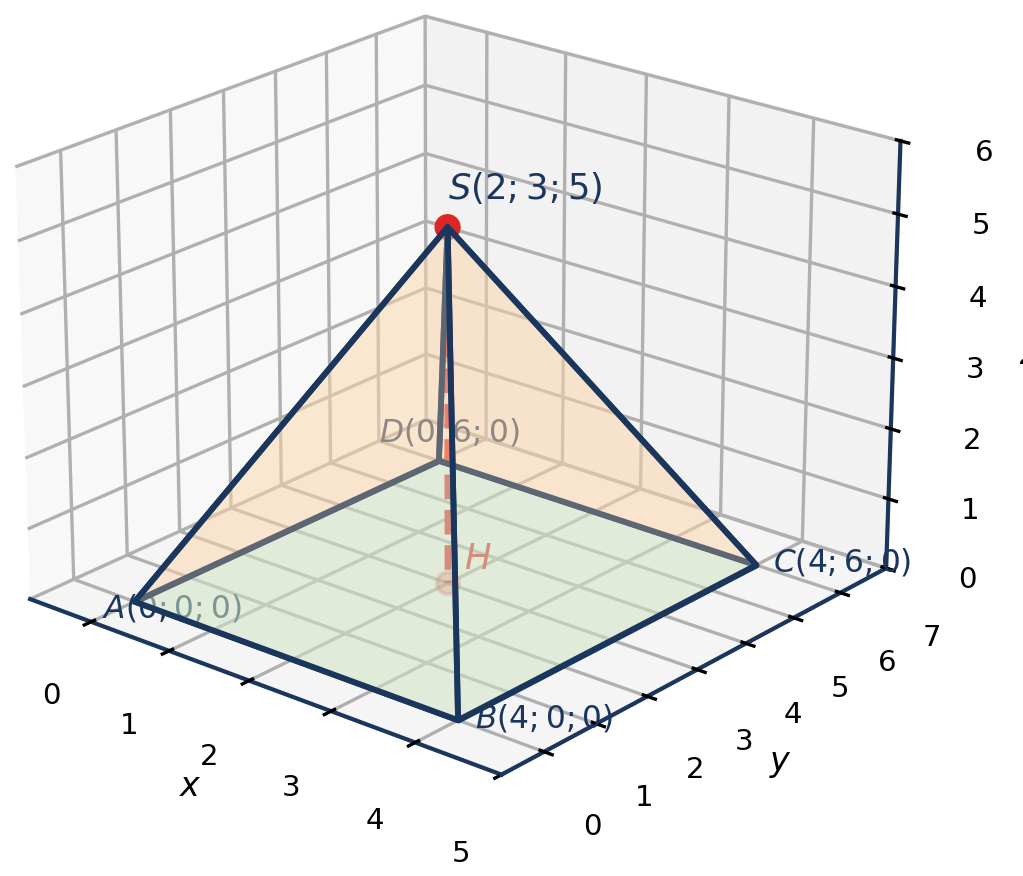
\includegraphics[width=\linewidth]{images/phan2_cau4_maivom_oxyz.png}
\end{minipage}

\end{enumerate}

% ==========================================
% PHẦN III
% ==========================================
\section*{PHẦN III. CÂU TRẮC NGHIỆM TRẢ LỜI NGẮN}
\textit{Thí sinh trả lời từ câu 1 đến câu 6. Điền đáp số theo quy chuẩn làm tròn được nêu trong từng câu.}

\begin{enumerate}[label=\textbf{Câu \arabic*:}, leftmargin=*]

\item \begin{minipage}[t]{0.56\linewidth}
Ông Bảo có một tấm tôn phẳng hình chữ nhật có kích thước $80\text{ cm} \times 50\text{ cm}$. Ông muốn chế tạo một chiếc thùng không nắp hình hộp chữ nhật để đựng đồ bằng cách cắt bỏ bốn hình vuông bằng nhau có cạnh $x\text{ (cm)}$ ở bốn góc tấm tôn rồi gập các mép tôn xung quanh lên. Tìm giá trị của $x$ (cm) để thể tích của chiếc thùng thu được đạt giá trị lớn nhất.
\end{minipage}\hfill
\begin{minipage}[t]{0.41\linewidth}
\vspace{-0.7\baselineskip}
\centering
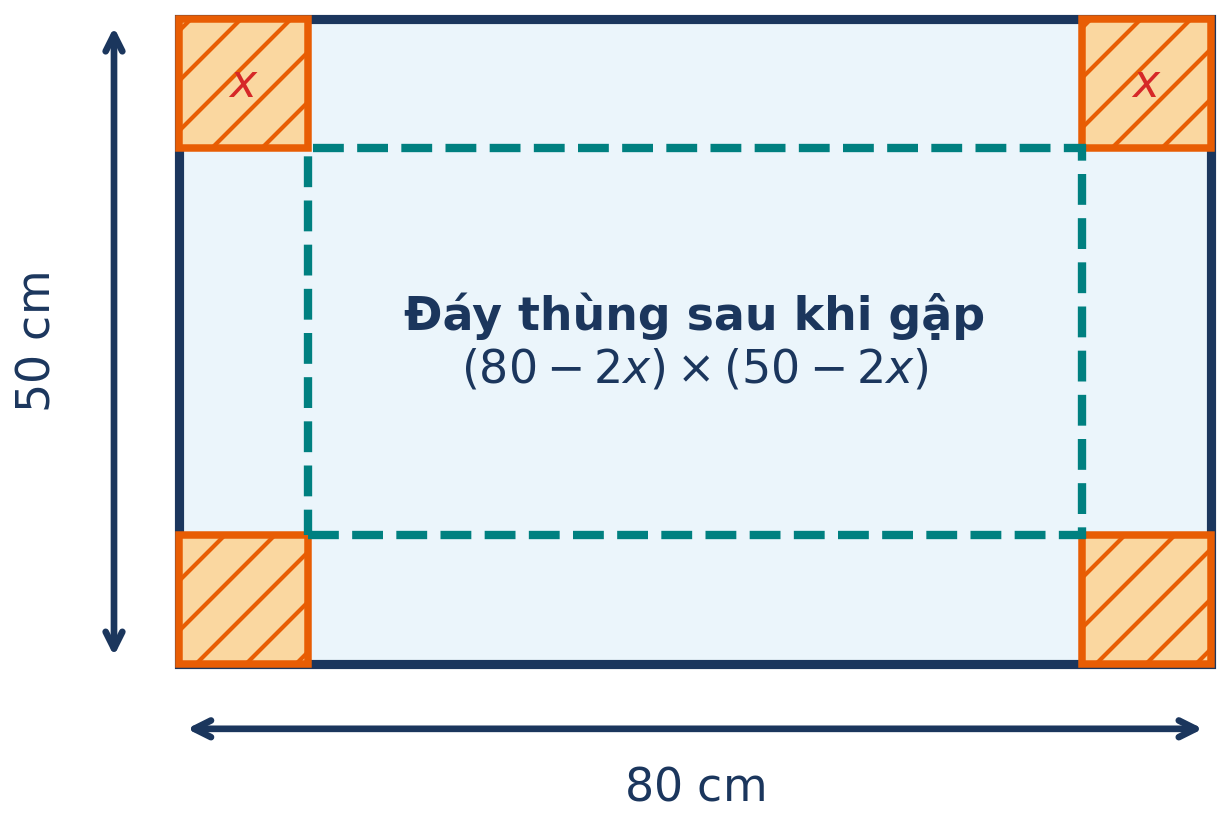
\includegraphics[width=\linewidth]{images/phan3_cau1_catton.png}
\end{minipage}

\item Chị Mai gửi tiết kiệm số tiền $800$ triệu đồng vào ngân hàng với mục đích tích lũy tài chính mua nhà. Ngân hàng áp dụng lãi suất cố định $6{,}5\%$/năm theo hình thức lãi kép nhập gốc hàng năm. Hỏi sau ít nhất bao nhiêu năm gửi tiền liên tục thì tổng số tiền cả gốc và lãi chị Mai thu được vượt quá $1{,}5$ tỷ đồng?
\begin{center}
    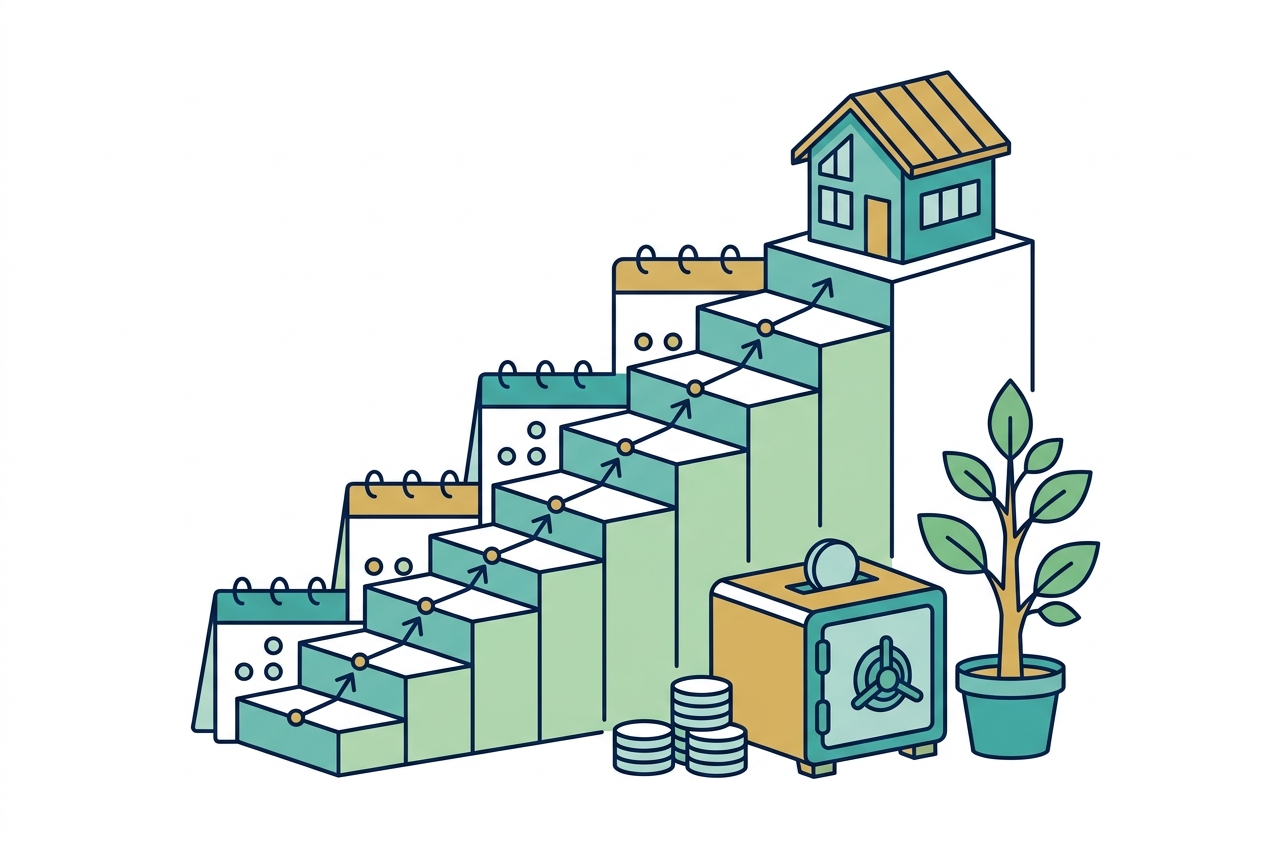
\includegraphics[width=0.42\linewidth,height=3.2cm,keepaspectratio]{images/phan3_cau2_tietkiem.jpg}
\end{center}

\item \begin{minipage}[t]{0.55\linewidth}
Một đài ra-đa kiểm soát hàng không đặt tại vị trí gốc tọa độ $O(0; 0; 0)$ trong hệ tọa độ $Oxyz$ (đơn vị trên các trục là km). Một chiếc máy bay thương mại đang bay chuyển động thẳng đều đi qua hai điểm mốc kiểm soát $A(1; 3; 2)$ và $B(5; 7; 6)$. Tìm khoảng cách ngắn nhất từ đài ra-đa $O$ đến đường bay của máy bay (làm tròn kết quả đến hàng phần mười của km).
\end{minipage}\hfill
\begin{minipage}[t]{0.42\linewidth}
\vspace{-0.7\baselineskip}
\centering
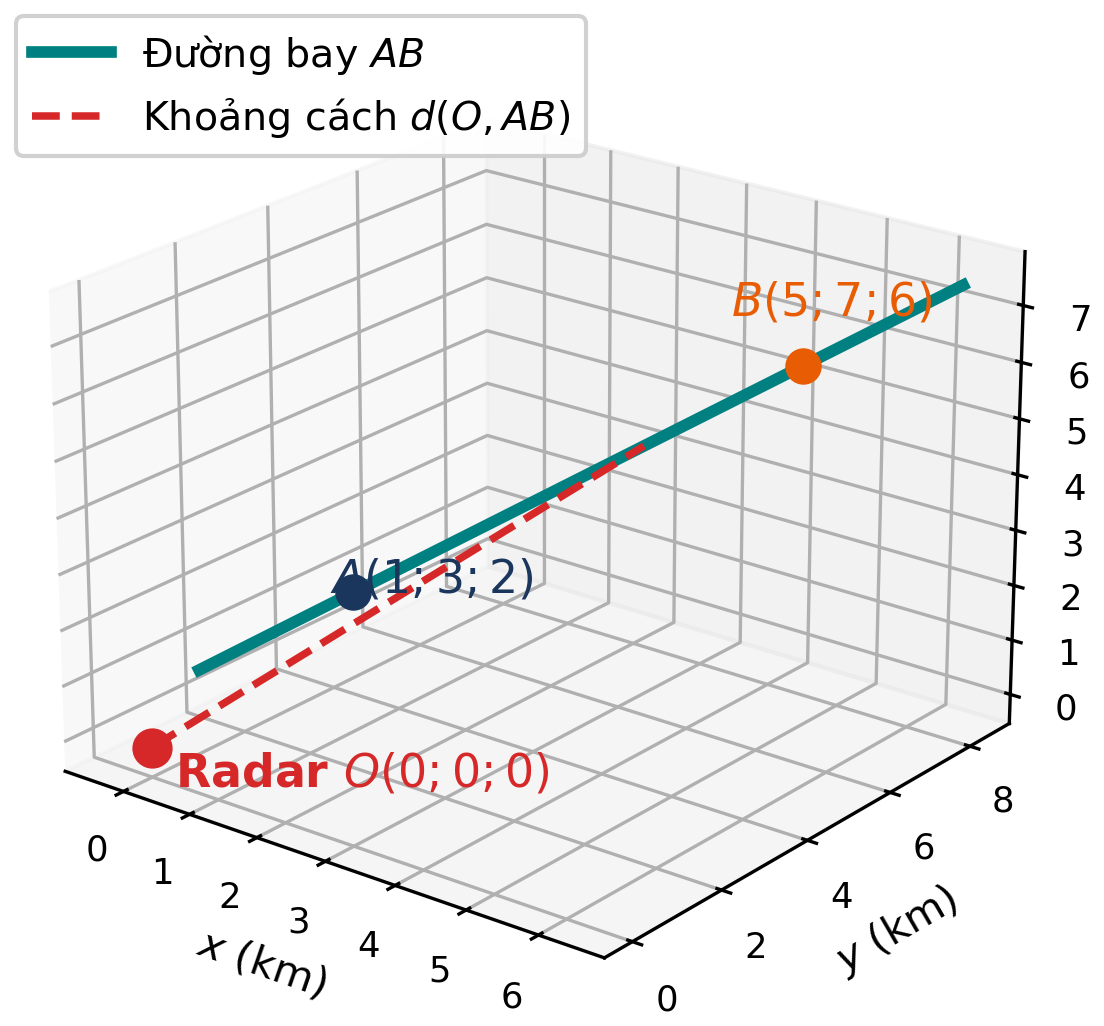
\includegraphics[width=\linewidth]{images/phan3_cau3_maybayradar.png}
\end{minipage}

\item Khảo sát số giờ tự học trong một tháng của $100$ học sinh khối 12 chuẩn bị thi tốt nghiệp thu được bảng số liệu ghép nhóm sau:
\begin{center}
\begin{tabular}{|c|c|c|c|c|c|}
\hline
\textbf{Số giờ tự học} & $[30; 40)$ & $[40; 50)$ & $[50; 60)$ & $[60; 70)$ & $[70; 80)$ \\ \hline
\textbf{Số học sinh} & $15$ & $25$ & $32$ & $20$ & $8$ \\ \hline
\end{tabular}
\end{center}
Tính tứ phân vị thứ ba $Q_3$ của mẫu số liệu ghép nhóm trên (làm tròn kết quả đến hàng phần mười).

\item Một xí nghiệp may mặc gia công sản phẩm trên 3 dây chuyền tự động $A, B, C$ với tỉ lệ sản lượng cung ứng lần lượt là $40\%$, $35\%$ và $25\%$. Tỉ lệ sản phẩm bị lỗi đường may của các dây chuyền $A, B, C$ tương ứng là $1{,}5\%$, $2\%$ và $3\%$. Chọn ngẫu nhiên một sản phẩm trong kho hàng chung để kiểm tra chất lượng. Tính xác suất để sản phẩm được chọn là sản phẩm bị lỗi đường may (kết quả viết dưới dạng số thập phân).
\begin{center}
    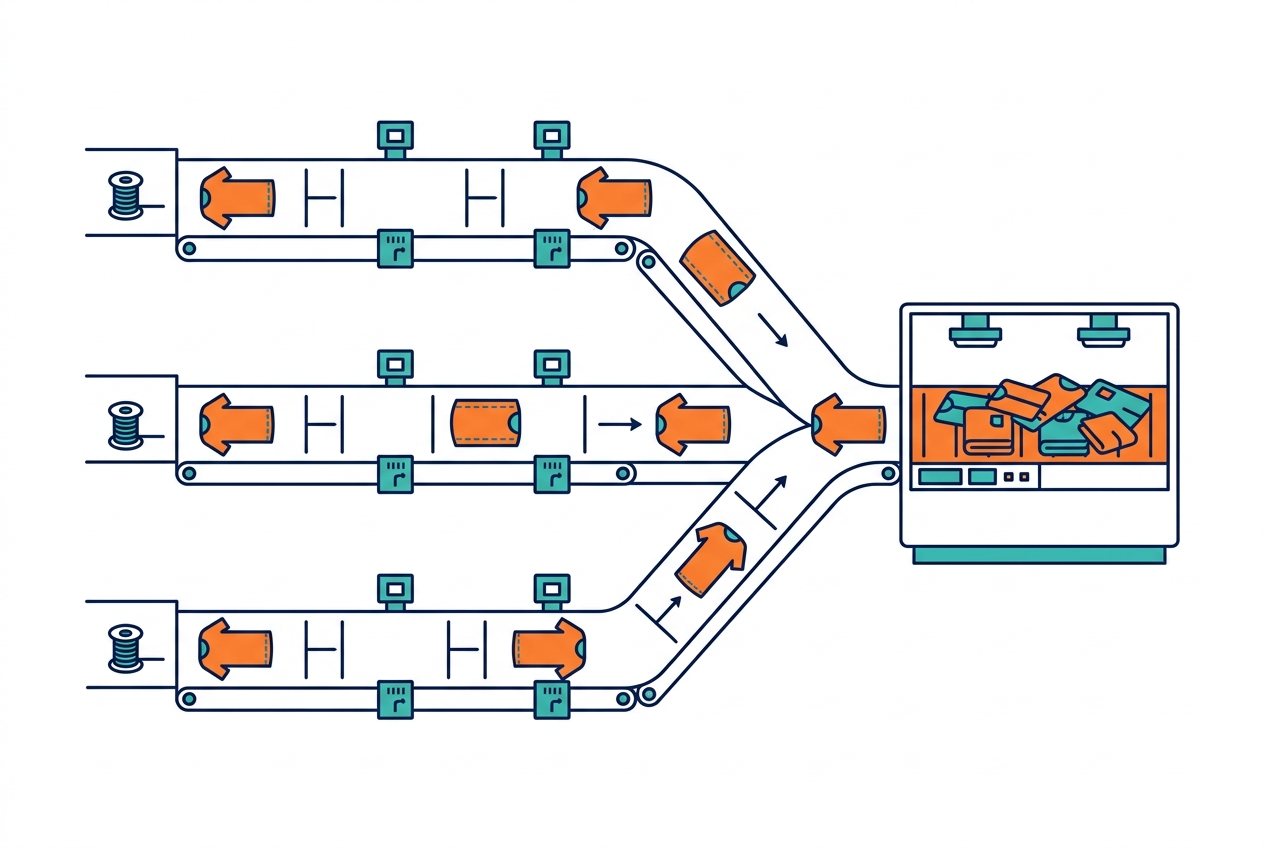
\includegraphics[width=0.42\linewidth,height=3.2cm,keepaspectratio]{images/phan3_cau5_daychuyenmay.jpg}
\end{center}

\item Trong một hội thi sáng tạo khoa học kỹ thuật, có 10 đề tài xuất sắc vào vòng chung kết gồm 4 đề tài về Trí tuệ nhân tạo (AI), 3 đề tài về Công nghệ sinh học và 3 đề tài về Vi mạch bán dẫn. Ban giám khảo chọn ngẫu nhiên 5 đề tài để trao giải thưởng. Tính xác suất để 5 đề tài được chọn có đủ cả 3 lĩnh vực và số đề tài AI đạt giải không vượt quá số đề tài Công nghệ sinh học đạt giải (làm tròn kết quả đến hàng phần trăm dưới dạng số thập phân).

\end{enumerate}

\newpage
% ==========================================
% BẢNG ĐÁP ÁN TỔNG HỢP
% ==========================================
\section*{BẢNG ĐÁP ÁN TỔNG HỢP}

\subsection*{1. PHẦN I}
\begin{center}
\begin{tabular}{|c|c||c|c||c|c||c|c|}
\hline
\textbf{Câu} & \textbf{Đáp án} & \textbf{Câu} & \textbf{Đáp án} & \textbf{Câu} & \textbf{Đáp án} & \textbf{Câu} & \textbf{Đáp án} \\ \hline
1 & A & 4 & D & 7 & B & 10 & B \\ \hline
2 & C & 5 & A & 8 & D & 11 & A \\ \hline
3 & B & 6 & C & 9 & C & 12 & D \\ \hline
\end{tabular}
\end{center}

\subsection*{2. PHẦN II}
\begin{center}
\begin{tabular}{|c|c|c|c|c|}
\hline
\textbf{Câu} & \textbf{Ý a)} & \textbf{Ý b)} & \textbf{Ý c)} & \textbf{Ý d)} \\ \hline
\textbf{1} & Đúng & Đúng & Sai & Đúng \\ \hline
\textbf{2} & Đúng & Đúng & Đúng & Sai \\ \hline
\textbf{3} & Đúng & Sai & Đúng & Sai \\ \hline
\textbf{4} & Đúng & Đúng & Đúng & Sai \\ \hline
\end{tabular}
\end{center}

\subsection*{3. PHẦN III}
\begin{center}
\begin{tabular}{|c|c||c|c||c|c|}
\hline
\textbf{Câu} & \textbf{Kết quả điền} & \textbf{Câu} & \textbf{Kết quả điền} & \textbf{Câu} & \textbf{Kết quả điền} \\ \hline
\textbf{1} & 10 & \textbf{3} & 1,4 & \textbf{5} & 0,0205 \\ \hline
\textbf{2} & 10 & \textbf{4} & 61,5 & \textbf{6} & 0,45 \\ \hline
\end{tabular}
\end{center}

\newpage
% ==========================================
% HƯỚNG DẪN GIẢI CHI TIẾT
% ==========================================
\section*{HƯỚNG DẪN GIẢI CHI TIẾT}

\subsection*{PHẦN I}
\begin{enumerate}[label=\textbf{Câu \arabic*:}, leftmargin=*]
\item \textbf{Đáp án A.}
Ta có $y = \dfrac{x^2 - x + 1}{x - 1} = x + \dfrac{1}{x - 1}$.\\
Đạo hàm: $y' = 1 - \dfrac{1}{(x - 1)^2} = \dfrac{(x - 1)^2 - 1}{(x - 1)^2} = \dfrac{x(x - 2)}{(x - 1)^2}$.\\
Cho $y' = 0 \iff x = 0$ hoặc $x = 2$.\\
Với $x = 0 \implies y(0) = -1 \implies A(0; -1)$.\\
Với $x = 2 \implies y(2) = 3 \implies B(2; 3)$.\\
Khoảng cách giữa hai điểm cực trị $A$ và $B$ là:
$$AB = \sqrt{(2 - 0)^2 + (3 - (-1))^2} = \sqrt{4 + 16} = \sqrt{20} = 2\sqrt{5}.$$

\item \textbf{Đáp án C.}
Đạo hàm: $y' = x^2 - 2mx + m^2 - 4 = 0$.\\
Ta có $\Delta' = m^2 - (m^2 - 4) = 4 > 0$ với mọi $m \in \mathbb{R}$. Do đó hàm số luôn có hai điểm cực trị phân biệt $x_1, x_2$.\\
Theo định lý Vi-ét: $\begin{cases} x_1 + x_2 = 2m \\ x_1 x_2 = m^2 - 4 \end{cases}$.\\
Theo giả thiết:
\begin{align*}
x_1^2 + x_2^2 &= (x_1 + x_2)^2 - 2x_1 x_2 = 4m^2 - 2(m^2 - 4) = 2m^2 + 8 = 26 \\
&\iff 2m^2 = 18 \iff m^2 = 9 \iff m = \pm 3.
\end{align*}
Vì $m \in \mathbb{Z}$ và $m \in [-10; 10]$, cả hai giá trị $m = 3$ và $m = -3$ đều thỏa mãn. Có đúng $2$ giá trị.

\item \textbf{Đáp án B.}
Bất phương trình $\log_2(x^2 - 2x + m) \le 3 \iff 0 < x^2 - 2x + m \le 2^3 = 8$.\\
Đặt $g(x) = x^2 - 2x$ trên đoạn $[0; 2]$. Ta có $g'(x) = 2x - 2 = 0 \iff x = 1 \in [0; 2]$.\\
Tính giá trị: $g(0) = 0$, $g(1) = -1$, $g(2) = 0 \implies \min_{[0; 2]} g(x) = -1$ và $\max_{[0; 2]} g(x) = 0$.\\
Để bất phương trình nghiệm đúng với mọi $x \in [0; 2]$, ta phải có:
$$\begin{cases} g(x) + m > 0 \\ g(x) + m \le 8 \end{cases} \iff \begin{cases} m > -\min_{[0; 2]} g(x) = 1 \\ m \le 8 - \max_{[0; 2]} g(x) = 8 \end{cases} \iff 1 < m \le 8.$$
Vì $m \in \mathbb{Z}$ và $m \in [-10; 10]$ nên $m \in \{2; 3; 4; 5; 6; 7; 8\}$. Vậy có đúng $7$ giá trị nguyên.

\item \textbf{Đáp án D.}
Vận tốc của chất điểm là:
$$v(t) = v_0 + \int_0^t a(u) du = \int_0^t (12 - 3u) du = 12t - 1{,}5t^2\text{ (m/s)}.$$
Vận tốc đạt giá trị lớn nhất khi $v'(t) = a(t) = 0 \iff 12 - 3t = 0 \iff t = 4\text{ giây}$.\\
Quãng đường chất điểm đi được từ $t = 0$ đến khi vận tốc đạt cực đại là:
$$S = \int_0^4 (12t - 1{,}5t^2) dt = \left[ 6t^2 - 0{,}5t^3 \right]_0^4 = 6(16) - 0{,}5(64) = 96 - 32 = 64\text{ m}.$$

\item \textbf{Đáp án A.}
Vectơ $\overrightarrow{CA} = (1; 2; -1 - z_0)$ và $\overrightarrow{CB} = (3; 0; 3 - z_0)$.\\
Tam giác $ABC$ vuông tại $C \iff \overrightarrow{CA} \cdot \overrightarrow{CB} = 0$:
$$1(3) + (-1 - z_0)(3 - z_0) = 0 \iff z_0^2 - 2z_0 = 0 \iff \left[\begin{aligned} z_0 = 0 \\ z_0 = 2 \end{aligned}\right.$$
Tổng các giá trị của $z_0$ bằng $0 + 2 = 2$.

\item \textbf{Đáp án C.}
Dân số sau $n$ năm là $P_n = P_0 (1 + r)^n = 2(1 + 0{,}015)^n = 2(1{,}015)^n$ (triệu người).\\
Để dân số vượt quá $2{,}5$ triệu người:
$$2(1{,}015)^n > 2{,}5 \iff (1{,}015)^n > 1{,}25 \iff n > \dfrac{\ln(1{,}25)}{\ln(1{,}015)} \approx \dfrac{0{,}22314}{0{,}01489} \approx 14{,}987.$$
Vì $n$ là số nguyên năm nên sau ít nhất $15$ năm.

\item \textbf{Đáp án B.}
Cỡ mẫu $N = 6 + 14 + 16 + 4 = 40$.\\
Giá trị đại diện các nhóm lần lượt là: $c_1 = 12$, $c_2 = 16$, $c_3 = 20$, $c_4 = 24$.\\
Số trung bình:
$$\bar{x} = \dfrac{6(12) + 14(16) + 16(20) + 4(24)}{40} = \dfrac{72 + 224 + 320 + 96}{40} = \dfrac{712}{40} = 17{,}8\text{ phút}.$$
Phương sai:
\begin{align*}
s^2 &= \dfrac{6(12 - 17{,}8)^2 + 14(16 - 17{,}8)^2 + 16(20 - 17{,}8)^2 + 4(24 - 17{,}8)^2}{40} \\
&= \dfrac{6(33{,}64) + 14(3{,}24) + 16(4{,}84) + 4(38{,}44)}{40} = \dfrac{478{,}4}{40} = 11{,}96.
\end{align*}
Độ lệch chuẩn $s = \sqrt{11{,}96} \approx 3{,}458 \approx 3{,}46\text{ phút}$.

\item \textbf{Đáp án D.}
Ta có $P(\overline{B}) = 1 - P(B) = 1 - 0{,}5 = 0{,}5$.\\
Theo công thức cộng xác suất:
$$P(A \cap B) = P(A) + P(B) - P(A \cup B) = 0{,}6 + 0{,}5 - 0{,}8 = 0{,}3.$$
Xác suất của biến cố $A \cap \overline{B}$ là:
$$P(A \cap \overline{B}) = P(A) - P(A \cap B) = 0{,}6 - 0{,}3 = 0{,}3.$$
Xác suất có điều kiện:
$$P(A|\overline{B}) = \dfrac{P(A \cap \overline{B})}{P(\overline{B})} = \dfrac{0{,}3}{0{,}5} = 0{,}6.$$

\item \textbf{Đáp án C.}
Vì bậc của tử số nhỏ hơn bậc của mẫu số nên đồ thị hàm số luôn có tiệm cận ngang $y = 0$.\\
Để đồ thị có đúng 3 đường tiệm cận thì phải có đúng 2 đường tiệm cận đứng.\\
Điều này tương đương với phương trình mẫu số $g(x) = x^2 - 2mx + 4 = 0$ có 2 nghiệm phân biệt khác 1:
$$\begin{cases} \Delta' = m^2 - 4 > 0 \\ g(1) = 1^2 - 2m(1) + 4 \ne 0 \end{cases} \iff \begin{cases} |m| > 2 \\ 5 - 2m \ne 0 \end{cases} \iff \begin{cases} m > 2 \text{ hoặc } m < -2 \\ m \ne 2{,}5 \end{cases}$$
Với $m \in \mathbb{Z}$ và $m \in [-5; 5]$, ta có $m \in \{-5; -4; -3; 3; 4; 5\}$. Có đúng $6$ giá trị nguyên.

\item \textbf{Đáp án B.}
Ta có $3^{x^2 - 4x} < 27 = 3^3 \iff x^2 - 4x < 3 \iff x^2 - 4x - 3 < 0 \iff 2 - \sqrt{7} < x < 2 + \sqrt{7}$.\\
Do đó $a = 2 - \sqrt{7}$ và $b = 2 + \sqrt{7} \implies a + b = 4$.

\item \textbf{Đáp án A.}
Bán kính mặt cầu là:
$$R = IA = \sqrt{(1 - 2)^2 + (1 - (-1))^2 + (2 - 0)^2} = \sqrt{1 + 4 + 4} = 3 \implies R^2 = 9.$$
Phương trình mặt cầu $(S)$ tâm $I(2; -1; 0)$ là $(x - 2)^2 + (y + 1)^2 + z^2 = 9$.

\item \textbf{Đáp án D.}
Thể tích khối tròn xoay là $V = \pi \int_1^2 (x - 1)^2 e^{2x} dx$.\\
Đặt $\begin{cases} u = (x - 1)^2 \\ dv = e^{2x} dx \end{cases} \implies \begin{cases} du = 2(x - 1) dx \\ v = \dfrac{1}{2} e^{2x} \end{cases}$.\\
Áp dụng công thức tích phân từng phần:
$$\int_1^2 (x - 1)^2 e^{2x} dx = \left[ \dfrac{(x - 1)^2 e^{2x}}{2} \right]_1^2 - \int_1^2 (x - 1) e^{2x} dx = \dfrac{e^4}{2} - \int_1^2 (x - 1) e^{2x} dx.$$
Tiếp tục đặt $\begin{cases} u_1 = x - 1 \\ dv_1 = e^{2x} dx \end{cases} \implies \begin{cases} du_1 = dx \\ v_1 = \dfrac{1}{2} e^{2x} \end{cases}$:
$$\int_1^2 (x - 1) e^{2x} dx = \left[ \dfrac{(x - 1) e^{2x}}{2} \right]_1^2 - \int_1^2 \dfrac{e^{2x}}{2} dx = \dfrac{e^4}{2} - \left[ \dfrac{e^{2x}}{4} \right]_1^2 = \dfrac{e^4}{2} - \left( \dfrac{e^4 - e^2}{4} \right) = \dfrac{e^4 + e^2}{4}.$$
Suy ra:
$$\int_1^2 (x - 1)^2 e^{2x} dx = \dfrac{e^4}{2} - \dfrac{e^4 + e^2}{4} = \dfrac{e^4 - e^2}{4} \implies V = \dfrac{\pi(e^4 - e^2)}{4}.$$
\end{enumerate}

\subsection*{PHẦN II}
\begin{enumerate}[label=\textbf{Câu \arabic*:}, leftmargin=*]
\item \textbf{Câu 1 (Kinh tế xưởng hóa chất):}
\begin{itemize}
    \item a) \textbf{Đúng}: Doanh thu khi bán $x$ trăm thùng phuy là $R(x) = x \cdot p(x) = x(111 - 3x) = 111x - 3x^2$ (triệu đồng).
    \item b) \textbf{Đúng}: Lợi nhuận ròng của doanh nghiệp là:
    $$L(x) = (111x - 3x^2) - (x^3 - 9x^2 + 60x + 40) - 15x = -x^3 + 6x^2 + 36x - 40\text{ (triệu đồng)}.$$
    \item c) \textbf{Sai}: Khi $x = 4$, lợi nhuận ròng là:
    \begin{align*}
    L(4) &= -(4)^3 + 6(4)^2 + 36(4) - 40 \\
    &= -64 + 96 + 144 - 40 = 136\text{ triệu đồng} \ne 150\text{ triệu đồng}.
    \end{align*}
    \item d) \textbf{Đúng}: Đạo hàm $L'(x) = -3x^2 + 12x + 36 = -3(x^2 - 4x - 12) = -3(x - 6)(x + 2)$.\\
    Với $x > 0$, ta có $L'(x) = 0 \iff x = 6$. Bảng biến thiên cho thấy hàm số đạt cực đại tại $x = 6$, với mức lợi nhuận lớn nhất bằng:
    $$L(6) = -(6)^3 + 6(6)^2 + 36(6) - 40 = 176\text{ triệu đồng}.$$
\end{itemize}

\item \textbf{Câu 2 (Thiết bị bay nghiên cứu khí quyển):}
\begin{itemize}
    \item a) \textbf{Đúng}: Vận tốc của thiết bị tại $t = 3\text{ s}$ là:
    $$v(3) = \int_0^3 a(t) dt = \int_0^3 (18t - 6t^2) dt = \left[ 9t^2 - 2t^3 \right]_0^3 = 9(9) - 2(27) = 27\text{ m/s}.$$
    \item b) \textbf{Đúng}: Độ cao đạt được tại thời điểm $t = 3\text{ s}$ là:
    $$h_1 = \int_0^3 v(t) dt = \int_0^3 (9t^2 - 2t^3) dt = \left[ 3t^3 - 0{,}5t^4 \right]_0^3 = 3(27) - 0{,}5(81) = 40{,}5\text{ m}.$$
    \item c) \textbf{Đúng}: Sau khi ngắt động cơ, thiết bị chuyển động chậm dần đều với gia tốc $a = -g = -10\text{ m/s}^2$. Thời gian bay thêm đến khi dừng lại ở đỉnh độ cao ($v = 0$) là:
    $$t_2 = \dfrac{v(3)}{g} = \dfrac{27}{10} = 2{,}7\text{ giây}.$$
    \item d) \textbf{Sai}: Độ cao bay thêm được là $h_2 = \dfrac{v(3)^2}{2g} = \dfrac{27^2}{20} = 36{,}45\text{ m}$.\\
    Tổng độ cao tối đa đạt được so với mặt đất là:
    $$H_{\max} = h_1 + h_2 = 40{,}5 + 36{,}45 = 76{,}95\text{ m} < 80\text{ m}.$$
\end{itemize}

\item \textbf{Câu 3 (Hệ thống AI sàng lọc bệnh):}
Gọi $A$ là biến cố ``Người được chọn mắc bệnh'' và $B$ là biến cố ``Kết quả sàng lọc dương tính''.\\
Theo bài ra: $P(A) = 0{,}02 \implies P(\overline{A}) = 0{,}98$. Độ nhạy $P(B|A) = 0{,}95$, độ đặc hiệu $P(\overline{B}|\overline{A}) = 0{,}90$.
\begin{itemize}
    \item a) \textbf{Đúng}: Xác suất người được chọn không mắc bệnh là $P(\overline{A}) = 1 - 0{,}02 = 0{,}98$.
    \item b) \textbf{Sai}: Tỉ lệ dương tính giả là $P(B|\overline{A}) = 1 - P(\overline{B}|\overline{A}) = 1 - 0{,}90 = 0{,}10 \ne 0{,}05$.
    \item c) \textbf{Đúng}: Theo công thức xác suất toàn phần:
    \begin{align*}
    P(B) &= P(A) \cdot P(B|A) + P(\overline{A}) \cdot P(B|\overline{A}) \\
    &= 0{,}02 \times 0{,}95 + 0{,}98 \times 0{,}10 = 0{,}019 + 0{,}098 = 0{,}117.
    \end{align*}
    \item d) \textbf{Sai}: Theo công thức Bayes, xác suất thực sự mắc bệnh khi nhận kết quả dương tính là:
    $$P(A|B) = \dfrac{P(A \cap B)}{P(B)} = \dfrac{0{,}02 \times 0{,}95}{0{,}117} = \dfrac{0{,}019}{0{,}117} \approx 0{,}1624 = 16{,}24\% < 20\%.$$
\end{itemize}

\item \textbf{Câu 4 (Mái vòm nhà thi đấu Oxyz):}
\begin{itemize}
    \item a) \textbf{Đúng}: Vì mặt sàn nằm trên mặt phẳng $z = 0$, hình chiếu vuông góc của đỉnh $S(2; 3; 5)$ lên sàn là điểm $H(2; 3; 0)$.
    \item b) \textbf{Đúng}: Chiều cao đỉnh mái so với sàn là $d(S, (ABCD)) = z_S = 5\text{ m}$.
    \item c) \textbf{Đúng}: Ta có $A(0; 0; 0), B(4; 0; 0), C(4; 6; 0), D(0; 6; 0)$ nên:
    \begin{align*}
    SA &= \sqrt{2^2 + 3^2 + 5^2} = \sqrt{38}\text{ m},\quad SB = \sqrt{(2-4)^2 + 3^2 + 5^2} = \sqrt{38}\text{ m}, \\
    SC &= \sqrt{(2-4)^2 + (3-6)^2 + 5^2} = \sqrt{38}\text{ m},\quad SD = \sqrt{2^2 + (3-6)^2 + 5^2} = \sqrt{38}\text{ m}.
    \end{align*}
    \item d) \textbf{Sai}: Hình chiếu của $SA$ lên mặt sàn là $HA$ với $HA = \sqrt{2^2 + 3^2} = \sqrt{13}\text{ m}$.\\
    Gọi $\alpha$ là góc giữa dây cáp $SA$ và mặt sàn:
    $$\tan\alpha = \dfrac{SH}{HA} = \dfrac{5}{\sqrt{13}} \approx 1{,}3867 > 1 = \tan 45^\circ \implies \alpha \approx 54{,}16^\circ > 45^\circ.$$
\end{itemize}

\end{enumerate}

\subsection*{PHẦN III}
\begin{enumerate}[label=\textbf{Câu \arabic*:}, leftmargin=*]
\item \textbf{Đáp số: 10.}
Sau khi cắt 4 hình vuông cạnh $x\text{ (cm)}$ ở bốn góc, đáy của chiếc thùng là hình chữ nhật có kích thước $(80 - 2x)\text{ cm}$ và $(50 - 2x)\text{ cm}$, chiều cao là $x\text{ (cm)}$ với điều kiện $0 < x < 25$.\\
Thể tích chiếc thùng là:
$$V(x) = x(80 - 2x)(50 - 2x) = 4(x^3 - 65x^2 + 1000x).$$
Đạo hàm:
$$V'(x) = 4(3x^2 - 130x + 1000) = 4(x - 10)(3x - 100).$$
Cho $V'(x) = 0 \iff x = 10$ hoặc $x = \dfrac{100}{3} \approx 33{,}3$ (loại vì không thuộc $(0; 25)$).\\
Bảng biến thiên cho thấy thể tích chiếc thùng đạt giá trị lớn nhất khi $x = 10\text{ cm}$.\\
Đáp số điền: \textbf{10}.

\item \textbf{Đáp số: 10.}
Số tiền gốc là $P_0 = 800$ triệu đồng, lãi suất hàng năm $r = 6{,}5\% = 0{,}065$.\\
Tổng số tiền cả gốc và lãi sau $n$ năm là $P_n = 800(1 + 0{,}065)^n = 800(1{,}065)^n$ (triệu đồng).\\
Yêu cầu $P_n > 1500$:
\begin{align*}
800(1{,}065)^n > 1500 &\iff (1{,}065)^n > 1{,}875 \\
&\iff n > \dfrac{\ln(1{,}875)}{\ln(1{,}065)} \approx 9{,}982.
\end{align*}
Vì số năm gửi là số nguyên nên chị Mai cần gửi ít nhất $10$ năm.\\
Đáp số điền: \textbf{10}.

\item \textbf{Đáp số: 1,4.}
Vectơ chỉ phương của đường bay đi qua $A(1; 3; 2)$ và $B(5; 7; 6)$ là:
$$\overrightarrow{AB} = (4; 4; 4) = 4(1; 1; 1) \implies \vec{u} = (1; 1; 1).$$
Vectơ vị trí từ đài ra-đa $O(0; 0; 0)$ đến mốc $A$ là $\overrightarrow{OA} = (1; 3; 2)$.\\
Tích có hướng:
$$\left[ \overrightarrow{OA}, \vec{u} \right] = (3 \cdot 1 - 2 \cdot 1;\; 2 \cdot 1 - 1 \cdot 1;\; 1 \cdot 1 - 3 \cdot 1) = (1; 1; -2).$$
Độ dài: $\left| \left[ \overrightarrow{OA}, \vec{u} \right] \right| = \sqrt{1^2 + 1^2 + (-2)^2} = \sqrt{6}$; độ dài $|\vec{u}| = \sqrt{1^2 + 1^2 + 1^2} = \sqrt{3}$.\\
Khoảng cách ngắn nhất từ đài ra-đa $O$ đến đường bay là:
$$d(O, AB) = \dfrac{\left| \left[ \overrightarrow{OA}, \vec{u} \right] \right|}{|\vec{u}|} = \dfrac{\sqrt{6}}{\sqrt{3}} = \sqrt{2} \approx 1{,}4142 \approx 1{,}4\text{ km}.$$
Đáp số điền: \textbf{1,4}.

\item \textbf{Đáp số: 61,5.}
Tổng số học sinh là $N = 15 + 25 + 32 + 20 + 8 = 100$.\\
Ta có $\dfrac{3N}{4} = \dfrac{3 \times 100}{4} = 75$.\\
Tần số tích lũy: nhóm 1 là 15; nhóm 2 là $15 + 25 = 40$; nhóm 3 là $40 + 32 = 72 < 75$; nhóm 4 là $72 + 20 = 92 \ge 75$.\\
Do đó nhóm chứa tứ phân vị thứ ba $Q_3$ là nhóm $[60; 70)$ với $L = 60$, độ dài nhóm $h = 10$, tần số nhóm $n_4 = 20$ và tần số tích lũy trước đó là $C = 72$.\\
Áp dụng công thức:
$$Q_3 = L + \dfrac{\dfrac{3N}{4} - C}{n_4} \cdot h = 60 + \dfrac{75 - 72}{20} \cdot 10 = 60 + \dfrac{30}{20} = 60 + 1{,}5 = 61{,}5\text{ giờ}.$$
Đáp số điền: \textbf{61,5}.

\item \textbf{Đáp số: 0,0205.}
Gọi $A, B, C$ lần lượt là biến cố sản phẩm do dây chuyền $A$, dây chuyền $B$, dây chuyền $C$ may.\\
Theo bài ra: $P(A) = 0{,}40$, $P(B) = 0{,}35$, $P(C) = 0{,}25$.\\
Gọi $L$ là biến cố ``Sản phẩm lấy ra bị lỗi đường may''.\\
Theo giả thiết: $P(L|A) = 0{,}015$, $P(L|B) = 0{,}02$, $P(L|C) = 0{,}03$.\\
Theo công thức xác suất toàn phần:
\begin{align*}
P(L) &= P(A) \cdot P(L|A) + P(B) \cdot P(L|B) + P(C) \cdot P(L|C) \\
&= 0{,}40 \times 0{,}015 + 0{,}35 \times 0{,}02 + 0{,}25 \times 0{,}03 = 0{,}006 + 0{,}007 + 0{,}0075 = 0{,}0205.
\end{align*}
Đáp số điền: \textbf{0,0205}.

\item \textbf{Đáp số: 0,45.}
Số phần tử của không gian mẫu là số cách chọn 5 đề tài từ 10 đề tài: $|\Omega| = C_{10}^5 = 252$.\\
Gọi $x, y, z$ lần lượt là số đề tài thuộc AI (có 4 đề tài), Sinh học (có 3 đề tài), Bán dẫn (có 3 đề tài) được chọn ($x + y + z = 5$).\\
Để được chọn đủ cả 3 lĩnh vực thì $x \ge 1, y \ge 1, z \ge 1$ và $x \le y$.\\
Vì $y \le 3, z \le 3$ nên ta có các trường hợp sau:
\begin{itemize}
    \item \textbf{Trường hợp 1}: $x = 1, y = 1 \implies z = 3$.\\
    Số cách chọn: $C_4^1 \cdot C_3^1 \cdot C_3^3 = 4 \times 3 \times 1 = 12$ cách.
    \item \textbf{Trường hợp 2}: $x = 1, y = 2 \implies z = 2$.\\
    Số cách chọn: $C_4^1 \cdot C_3^2 \cdot C_3^2 = 4 \times 3 \times 3 = 36$ cách.
    \item \textbf{Trường hợp 3}: $x = 1, y = 3 \implies z = 1$.\\
    Số cách chọn: $C_4^1 \cdot C_3^3 \cdot C_3^1 = 4 \times 1 \times 3 = 12$ cách.
    \item \textbf{Trường hợp 4}: $x = 2, y = 2 \implies z = 1$.\\
    Số cách chọn: $C_4^2 \cdot C_3^2 \cdot C_3^1 = 6 \times 3 \times 3 = 54$ cách.
\end{itemize}
Tổng số trường hợp thuận lợi là:
$$N = 12 + 36 + 12 + 54 = 114\text{ cách}.$$
Xác suất cần tìm là:
$$P = \dfrac{114}{252} = \dfrac{19}{42} \approx 0{,}4524 \approx 0{,}45.$$
Đáp số điền: \textbf{0,45}.
\end{enumerate}

\end{document}
